%\title{Title page with logo}
%----------------------------------------------------------------------------------------
%	PACKAGES AND OTHER DOCUMENT CONFIGURATIONS
%----------------------------------------------------------------------------------------

\documentclass[12pt]{report}

%Font and Language
\usepackage[english]{babel}
\usepackage[utf8]{inputenc}
\usepackage{amsmath,amsfonts,amssymb}
\RequirePackage{lmodern}
\RequirePackage[scaled]{helvet}
\RequirePackage[T1]{fontenc}
\RequirePackage{lettrine} 
\usepackage{a4wide}

%Grpahics
\usepackage{graphicx}
\usepackage[colorinlistoftodos]{todonotes}

% Bibliography
\RequirePackage[babel]{csquotes}
\RequirePackage[backend=biber, style=numeric-comp,maxnames=99,maxalphanames=5]{biblatex}
\usepackage[algo2e]{algorithm2e} 

%for sideways pictures
\usepackage{rotating}

\setlength{\parindent}{0pt}


\addbibresource{mybib.bib}

\begin{document}

\begin{titlepage}

\newcommand{\HRule}{\rule{\linewidth}{0.5mm}} % Defines a new command for the horizontal lines, change thickness here

\center % Center everything on the page
 
%----------------------------------------------------------------------------------------
%	HEADING SECTIONS
%----------------------------------------------------------------------------------------

\textsc{\LARGE University of Applied Sciences Ulm}\\[1.5cm] % Name of your university/college
\textsc{\Large Robocup Logistics League}\\[0.5cm] % Major heading such as course name
\textsc{\large Smartbots Ulm}\\[0.5cm] % Minor heading such as course title

%----------------------------------------------------------------------------------------
%	TITLE SECTION
%----------------------------------------------------------------------------------------

\HRule \\[0.4cm]
{ \huge \bfseries Technical Report}\\[0.4cm] % Title of your document
\HRule \\[1.5cm]
 
%----------------------------------------------------------------------------------------
%	AUTHOR SECTION
%----------------------------------------------------------------------------------------

\begin{minipage}{0.4\textwidth}
\begin{flushleft} \large
\emph{Author:}\\
Thomas \textsc{Bockmair} \\% Your name
Maximilian \textsc{Heichler} \\% Your name
Barbara \textsc{Roessle} \\% Your name
\end{flushleft}
\end{minipage}
~
\begin{minipage}{0.4\textwidth}
\begin{flushright} \large
\emph{Supervisor:} \\
Dr. Christian \textsc{Schlegel} % Supervisor's Name
\end{flushright}
\end{minipage}\\[2cm]

% If you don't want a supervisor, uncomment the two lines below and remove the section above
%\Large \emph{Author:}\\
%John \textsc{Smith}\\[3cm] % Your name

%----------------------------------------------------------------------------------------
%	DATE SECTION
%----------------------------------------------------------------------------------------

{\large \today}\\[2cm] % Date, change the \today to a set date if you want to be precise

%----------------------------------------------------------------------------------------
%	LOGO SECTION
%----------------------------------------------------------------------------------------

\includegraphics{pic/logo.png}\\[1cm] % Include a department/university logo - this will require the graphicx package
 
%----------------------------------------------------------------------------------------

\vfill % Fill the rest of the page with whitespace

\end{titlepage}

\tableofcontents
\listoffigures
\listoftables
%\listofalgorithms


%\section{Abstract}
\begin{abstract}
	The students of the masters program "Information Systems" of the University of Applied Sciences Ulm are participating at the RoboCup German Open since 2010. This year, the third attending at the RoboCup Logistics League takes place. The Logistics League covers the requirements of the industry factories of the future. Robots have to interact autonomously with the environment, which includes to explore production machines, areas of the environment and react on different kinds of actions and events.\
This report gives insights into the current state of the project RoboCup. It describes the components, which will be used in the upcoming RoboCup 2018 in Magdeburg. The report helps the junior members to get into the project and provides an overview on the whole project state.


\end{abstract}

\chapter{Introduction}
	\subsection{Motivation}

In the masters program "Informationsysteme" of the University of Applied Sciences Ulm, each student gets hand on experience in developing and implementing software in a group project by participating in a project lasting two semesters. One of the projects is the robotics project in the service robotic research laboratory of the University of Applied Sciences Ulm headed by Prof. Dr. Christian Schlegel. The service robotic research laboratory is focused on research in the field of methods, algorithms and software tools for implementing service robots and autonomous systems for everyday use. \\
For several years students of the masters course participated in the robotics project. The project is focused on industrial robots and the students gather theoretical and practical experience in working, developing and implementing software for service robots. Each project includes the participation in the RoboCup German Open (RGO) where students from universities all over the world come together and compete against each other in different contests. The SmartBots@Ulm, the project team of the masters course "Informationssysteme" of the University of Applied Sciences Ulm participated in the RoboCup German Open 2017 in the RoboCup Logistics League (RCLL). It focuses on in-factory logistical applications to simulate a modern industrial working environment. The robots autonomously fulfill tasks and produce working output. This section is of enormous interest since it covers the idea of the changing industry environment towards digitalisation and industry 4.0 requirements. \\
The project not only included gaining experience in developing and implementing software for service robots but also gaining the experience of working in a long term group project and organizing the project as a team. The tasks of the group project were not only developing software and putting it together but also being organized and work collaboratively as a team with defined roles and activities, which included the organization of the participation of the RoboCup German Open, managing the residence, renting cars, signing insurances and handling the financial situations to successfully participate in the contest. 

\subsection{Objective}

This technical report provides basic information on the current state of the software, components and deployments of the robotinos used in the RoboCup German Open 2017. At first, there is a small overview of the principles of the RoboCup German Open 2017 and the difficulities the teams had to face. The next chapter gives insights on the current state of the used components and the way they work and interact together. All the components are explained, including the adjustments on top of the version of the last team, and the difficulties which have been faced. The teams lessons learned are stated in the subsequent chapter and the last chapter is about the ideas and open topics for next years student team

\chapter{Robocup Logistic League}
	\section{Overview}

The Logistic Leagues of the Robocup is a relative new league. The topic of this Robocup league is the upcoming Industry 4.0. Two teams are participating in each game, which consists of three phases: Setup Phase, Exploration Phase and Production Phase. Every team is allowed to participate with up to three robots, which have to fulfill the tasks of the league autonomously. There are 14 so called MPS stations on the field. So each team has seven machines assigned. The robots have to interact with those machines in the Exploration Phase and in the Production Phase.

\begin{figure}%[tbhp]
\centering
\includegraphics[width=\linewidth]{pic/field.png}
\caption{Field for robocup 2017}
\label{fig:frog}
\end{figure}

The following shortly describes the three phases of the league. For detailed information, the actual Rulebook  \cite{RC17} of the league is a must.

\paragraph{Setup Phase:}
The Setup Phase lasts five minutes. The team has time to setup their robots for the Exploration Phase and the Production Phase. After the five minutes the Referee Box will start the next phase automatically.

\paragraph{Exploration Phase:}
The Exploration Phase is the second phase in the Robocup Logistics League. The robots have three minutes to explore the field and find their seven MPS stations. They have to report each station to the Referee Box. The report contains the machine name (encoded in the ALVAR Tag), the zone where the machine is located, and the orientation of the machine in degrees. After the three minutes, the Referee Box starts the Production Phase.

\paragraph{Production Phase:}
The Production Phase is the main game phase of the Logistics League. It lasts 17 minutes and is quite complex. The Referee Box publishes information which includes machine zones and orientations, also colors of ring and cap stations. That information is needed to play the Production Phase. The Referee Box then orders products, which are assembled by the MPS stations. The robots have to bring the pieces of the ordered product to the production machines and deliver it finally to a Delivery Station.


\section{Changes in 2018}

The Smartbots@Ulm team will participate in the Robocup German Open 2018 in Magdeburg. Like the last two years, the team is preparing for the Logistics League. The changes in the Rulebook are expected to be small. A new storage station will be available on the field. More specific information is not available right now, but should be published in time for the Magdeburg event at \url{http://www.robocup-logistics.org/rules}.


\section{Lessons Learned of Robocup 2017}

In the year 2017 it was not clear how to setup the network for the game phases. The hosts of the Logistics League provide two configurations: one for testing and one for participating in the game. For that it is recommended to speak with the hosts at the Robocup to set up the network properly.


\section{Robocup Logistics League Participation}

This year it will be possible to play a complete Exploration Phase. The team will participate with one robot, which is able to detect stations, dock to stations and scan their ALVAR-tags. It will send the information back to the Referee Box and to finally earn points. Maybe the team will configure the SmartInstructionPlanner component at the Robocup in a way, that three robots participate at the game. The Production Phase is not implemented yet, so the team plans to skip the third phase.


\chapter{Components}

\section{Overview}
	This chapter gives an overview on the current states of the particular components. The \textit{Refbox} component and the \textit{SmartAlvarTagDetection} component will be just recapped shortly, because just minimal changes were made.
The new components \textit{SmartRobotinoDetection}, \textit{SmartRobotinoMPSDocking}, \textit{SmartRobotinoInstructionPlanner} and a new implementation of the sequence of tasks in the \textit{LispServer} are explained in detail in this chapter.

	
\section{SmartRobotinoInstructionPlanner}
	

\subsection{Overview}
The instruction planner is placed at the top layer of the whole SmartSoft architecture,
therefore it is meant to be the "Swarm Manager" of all Robots that work on a common Task. \\
This approach has been split up into two different aspects, one part of the Instruction planner has to
observe all robots and the states that they are currently in, as well as the task that they are working on.
While the other part of the Instruction planner needs to keep up with the progress on the objective, to
predict and estimate the proximate steps to the goal.

\subsection{Idea}

The following Picture \ref{fig:instr_overview} shows the internal structure of the
instruction planner.
As seen in the Picture the instruction planner will do multiple things: \newpage
In Blue:\\
\begin{itemize}
    \item \textbf{Game Management:}  organization of next steps
    \begin{itemize}
        \item Exploration Management
            \begin{itemize}
                \item keeps log of found machines
                \item estimates explorable positions
                \item suggests next orders to reach the objective
            \end{itemize}
        \item Production Management
        \begin{itemize}
            \item coming up
        \end{itemize}
    \end{itemize}
    \item \textbf{Fleet Management:} organization of robots and their progress
    \begin{itemize}
        \item which state they are in (e.g disqualified / maintenance / active)
        \item what they are working on
        \item error handling
    \end{itemize}
\end{itemize}

\begin{figure}[h]
\centering
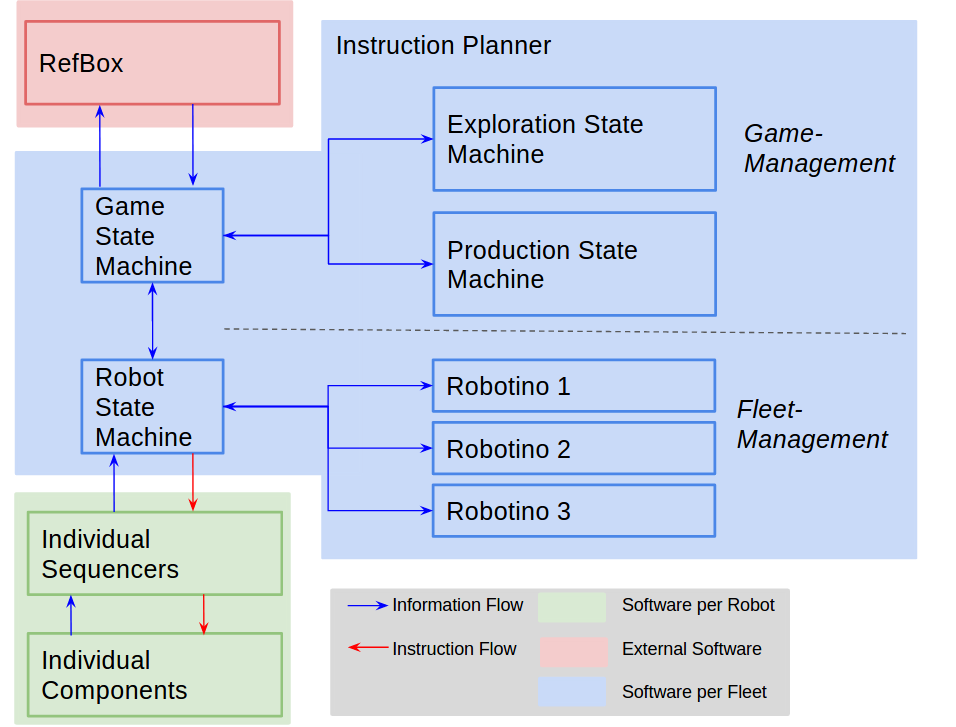
\includegraphics[scale=0.23]{pic/Instructionplanner2018.png}
\caption{Management of Robot Swarm and the Objective}
\label{fig:instr_overview}
\end{figure}
\newpage

Since the Blue-part of figure \ref{fig:instr_overview} handles the internal management
it can be treated at as an agent that provides the next orders for the robots, based
on their actual situation.\\
This situation is brought into the instruction planner via the Sequencers of each
robot.
In Green: \\
\begin{itemize}
    \item \textbf{Sequencers}
    \begin{itemize}
        \item handle all events on robot
        \item local management of robot
    \end{itemize}
    \item \textbf{Components}
    \begin{itemize}
        \item actual hardware
        \item creates events
    \end{itemize}
\end{itemize}


\subsubsection{Objective Management}
The objective management consists of multiple \textit{state machine}, that are in
a hierarchical order.
All state machines listen to the events that are received via the \textit{sequencers}, or
the \textit{refbox}.
The thought behind this architecture is an intelligent agent that can be "asked" for the next
best step to take.\\

The game state machine is a first level state machine that takes care of the current
game phase, (e.g. exploration phase, production phase, pause, etc. ). depending on the phase the
events are then forwarded to the next level state machines, such as the exploration state machine. \\
\\
The exploration state machine takes then care of all objectives that have to be fulfilled in the
exploration phase.
\subsubsection{Fleet Management}


The

\subsection{Changes}
Previously the purpose of the instruction planner was misunderstood, so the whole structure of
this component had to be planned again. \\
The implementation now differs a lot from the old of 2017. Only view lines of code could be recycled and used again.
A completely new system has been introduced: the \textit{hierarchical state machines}. The implementation of
this system now is more modular, parts (e.g. the state machines for the phases) can easily be exchanged and
replaced with other approaches or implementations. \\
Also new is the split of tasks into \textit{Fleet Management} and \textit{Objective Management}. This
allows the system to be even more flexible, since commendation of the robot is now isolated from the Task that the
Swarm should perform. \\
\\
Overall the instruction planner has been completely redesigned and is still under construction.
The basic ideas are implemented but still need to be filled with "live".

\subsection{Conclusion}
With the new architecture of the instruction planner multiple new features can be implemented.
\begin{itemize}
    \item \textbf{Multiple Robots} The new implementation would allow the use of multiple robots on the field, since
    the new architecture considers the use of multiple sequencers.
    \item \textbf{Intelligent Agents} The \textit{Objective Management} is designed to work with agents that can be asked
    for the next steps, in the actual case the implementation works with state machines. Other implementations of Agents can
    also be fit into the interface.
    \item \textbf{divide et impera} Separating the robot management form the objective management separates two problems
    that can be handled individually: \textit{Objective Manager} creates the next task and the \textit{Fleet Manager} takes care
    of all robots and assigns this task to the best candidate.
\end{itemize}

The actual level of Production does not contain a fully functional instruction planner.
The current state consists of the skeleton of the parts, the implementation of the
actual agent is missing as well as the logic to distribute the tasks to multiple Robots.
The Architectural changes allow to start the work on any part of the system since the would not affect each other,
while still just some implementation is necessary for the whole code to work.
Probably the first implementations of the \textit{Objective Manager} might be a
simple static implementation of a point pattern to follow, as well as a simple \textit{Fleet Manager} that
assigns just one order at a time to only onre Robot.


\subsection{Testing}
The instruction planner is still under construction and therefore untested.
Especially the use of Multiple Robotinos could not be tested and is not planned to take action in the upcoming contest.

\newpage


\section{LispServer/Sequencer}
	This section describes the new LispServer or Sequencer component. It is a special component, because the Sequencer is placed on a different coordination level in SmartSoft. The other components (e.g. Detection, Docking, ALVAR Detection) are placed in the Skill Layer of SmartSoft, and the Sequencer is placed in the Sequencing Layer. In the Sequencing Layer, the developer can model different scenarios, and trigger or call the Skill Level components to satisfy a specific or well designed task. 
For the Robocup 2018, the whole Exploration Phase was modeled in the Sequencing Layer.

\subsubsection{Overview}
\label{sec:sequencer_overview}
The so called Sequencer is a central building block of SmartSoft and is responsible for assigning decision-spaces to the components on the skill layer \cite{SmartSoftManual}. In the case of the RoboCup, it manages the whole sequence of actions of the Exploration Phase (drive to a point in the field, detect stations, dock to stations, take a picture and detect the ALVAR tag, send information back to the instruction planner). This sequence of actions is shown in figure \ref{fig:sequ_overview}.
The entities in the Sequencer (Approach Location, Detect MPS, Dock MPS, ALVAR TAG) are the different .lisp files, which the Sequencer executes.

\begin{figure}[h]
\centering
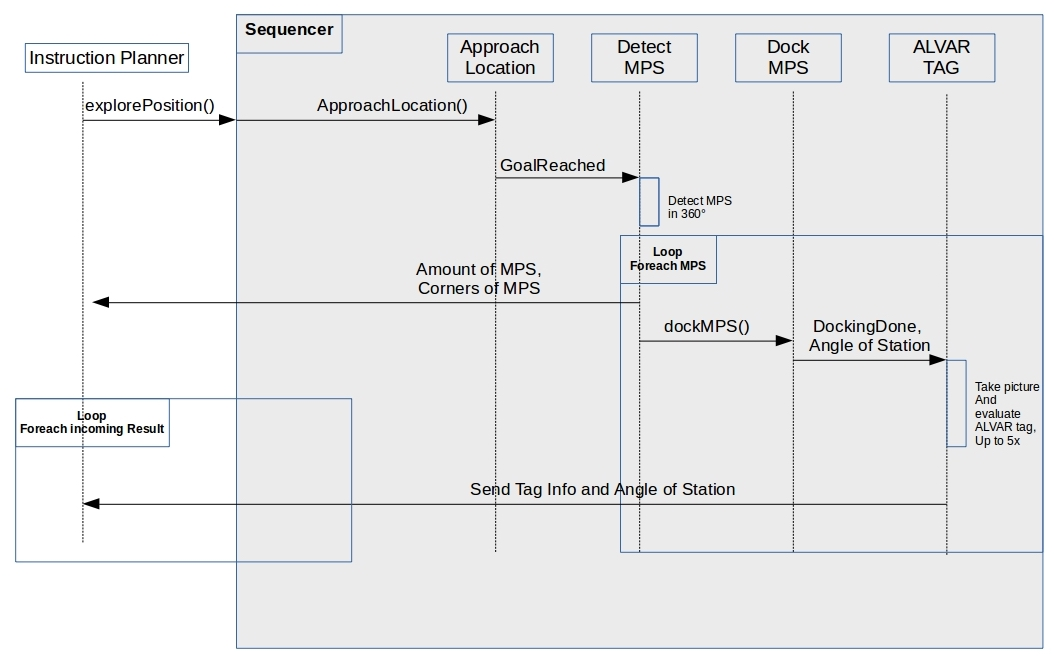
\includegraphics[scale=0.5]{pic/sequenceSequencer.jpg}
\caption{Sequence of the implemented Exploration Phase in the Sequencer}
\label{fig:sequ_overview}
\end{figure}


\subsubsection{Procedure of the Exploration Phase}

The sequence of actions and the calling or triggering of the skill components are implemented in .lisp files.

\begin{itemize}

\item ExplorePosition

The InstructionPlanner starts the Exploration Phase in the Sequencer by calling the \textit{explorePosition()} method. This is the entry point for the sequence of actions for the Exploration Phase. The robot will drive to a predefined position on the field, which is managed by the InstructionPlanner.  

\item Detect MPS

After reaching the position, the robot will perform the detection of the MPS stations. The sequencer triggers the component SmartRobotinoDetection.
Each detected MPS station is sent back to the Sequencer, which manages a list of the detected MPS stations. 
The Sequencer sends the amount of detected MPS stations back to the InstructionPlanner. This is necessary, because the Instruction Planner needs to know, for how much results he is waiting for, before a new \textit{explorePosition()} command is sent.
For every detected MPS, the Sequencer triggers the SmartMPSRobotinoDocking component.

\item Dock MPS

The SmartMPSRobotinoDocking component tries to dock to the appropriate machine. 
The Docking component gives feedback, whether the docking was successful or not. By telling the Sequencer \textit{Docking done (e.g. success)}, the Alvar Tag Detection component is triggered. This triggering message holds also the angle of the machine, which was calculated in the docking component.

\item ALVAR Tag Detection

The last part of the chain is the ALVAR Tag Detection. It provides an ALVAR Tag, or an error message. 
If an ALVAR Tag gets detected, the Sequencer sends back the angle of the station (from the docking component) and the ALVAR Tag information to the Instruction Planner.

\end{itemize}

\subsubsection{Conclusion }

By implementing the Exploration Phase (and also the Production Phase later on) in the Sequencing Layer, the big disadvantage of the Instruction Planner design of the former team is solved. The Instruction Planner of 2017 tried to absorb the functionality of the Sequencer of SmartSoft, by implementing a state machine, which represented the Exploration Phase completely (detection, docking, ALVAR tag detection) (\ref{ch:SmartRobotinoInstructionPlanner}).
Unfortunately there was not enough time for the team 2018 to implement also the Production Phase in the Sequencer.



	
\section{SmartAlvarTagDetection}
	The following chapter is about the old SmartAlvarTagDetection component. It is only a brief description of the component and for more details the Technical Report of 2017 is recommended. 

\subsubsection{Overview}


The SmartAlvarTagDetection is implemented by the former Robocup team. The component is a crucial component because it identifies the Alvar Tags on the MPS machines. With those Alvar Tags, the robot can identify the machine name and wether the robot is facing the front or back side of the machine. The actual component deals with four types of the MPS machines: Base Station, Cap Station, Ring Station and Storage Station. Therefor a lookup table in the component holds 14 machines with 28 unique Alvar Tags.
For the Robocup 2018 a new Storage Station is announced. Because there is no new rulebook available yet, it is not quite clear if a new Alvar Tag is needed.

\begin{figure}[h]
\centering

\includegraphics[scale=0.75]{pic/numberedMarker.png}
\caption{Shows an AlvarTag with corresponding ID}
\label{fig:smartAlvarFlow}
\end{figure}

To identify the Alvar Tag, a webcam is used to take a picture of the tag. The picture is evaluated by an algorithm, offered by the Alvar Library, which maps the tag to and specific ID. If the deposited lookup table in the component holds the ID of the scanned Alvar Tag, the appropriate marker is returned. Markers hold the information about the color of the owning team, type of station and the side (front or back). 


\subsubsection{Changes in 2018}

Because the component worked well at the Robocup 2017, only minimal adjustments were made. The version of 2017 returns after one evaluation of the Alvar Tag with a message whether a tag was found or not. The Instruction Planner kept triggering the component up to five times, to ensure that the reason for no tag ID is not the quality of the picture. 
This repetition, done by the Instruction Planner is now moved in the SmartAlvarTagDetection component. Because the task of the component is to offer an ID out of an AlvarTag, it is reasonable to repeat the procedure up to a maximum (five times) in the component itself.


\subsubsection{Testing}

The component can still be tested in the isolated DeployAlvarTest deployment. Because of the minimal changes in the component it was not necessary to test the component in a isolated deployment. The new component is integrated in the masterdeployment for the Robocup 2018 and has been tested there. It found in most of the cases the correct ID of the AlvarTag on the machine.
The former team has tested the component in the DeployAlvarTest deployment. Their outcome was that the distance of the webcam to an AlvarTag should not be more than six meters. The angle to the AlvarTag from the webcam should not be more than 45 or 120 degree.
	
\section{Refbox}
The Refbox has not changed since 2017. 


\subsubsection{Overview}

The referee of the Logistic League is a machine, which is implemented in an external component. This component is called the Referee Box (Refbox) and is implemented by the Unversity Aachen. The Refbox communicates with the robots of both teams and the MPS Stations during a game. It manages the different phases of the game and handles the points of each team. The manual of the Refbox is located at  \url{http://www.robocup-logistics.org/refbox}.

The Refbox did not changed since the last Robocup 2017. Therefor this chapter summarizes the most important steps to work with the Refbox. For more detailed information, the Technical Report of 2017 is recommended.


\subsubsection{Configuration}

The Refbox is installed on the Laptop of the Robocup team in the laboratory. To run the Refbox, two programs are needed: llsf-refbox and llsf-refbox-shell. The actual Refbox program is the llsf-refbox implementation. The llsf-refbox-shell is like the name says, the graphical user interface for the Refbox.

The Referee Box can be configured via the “config.yaml” file. The most important adjustments in the file are the IP addresses. 
 
 \begin{figure}[!h]
\centering
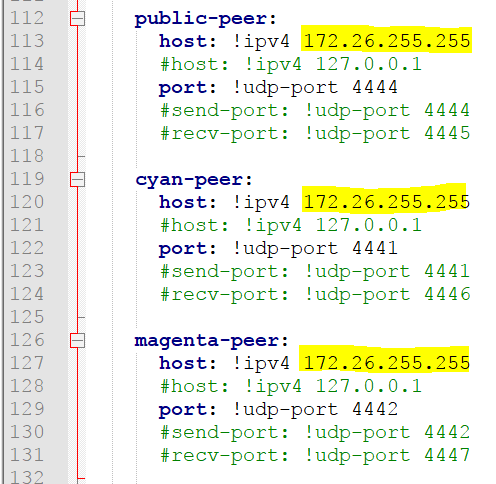
\includegraphics[]{pic/config_file_1.png}
\caption{IP adresses to modify in the config.yaml file}
\label{fig:configFile1}
\end{figure}

The other configuration refers the name of the team and their crypto key. 

\begin{figure}[!h]
\centering
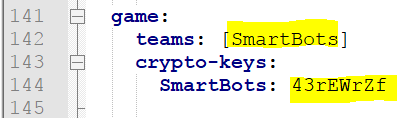
\includegraphics[]{pic/config_file_2.png}
\caption{Name and key to modify in config file}
\label{fig:configFile2}
\end{figure}

The crypto key must be the same like the key in the RefboxServer component. Therefor at the Robocup the team may adjust in the RefboxServer component the crypto key. The hosts of the game will offer a key for each team.



\section{SmartLogisticsRefboxServer}
	The component SmartLogisticsRefboxServer has only been modified to also send the rotation of a MPS during the implementation process.
Therefore this chapter also just summarizes the functionality of the component and it is again recommended to read the Technical Report of 2017 for more specific information.

\subsubsection{Overview}

The component handles the communication between the physical Refbox and the robots. The Refbox uses Google Protocol-Buffers for message serialization. Therefor a component is introduced to act as an interface between the physical Refbox and the robots on the field. The task of the component is to receive Google Protocol-Buffers messages from the Refbox and map them into TCL-messages of Smartsoft. Then it sends the TCL-message to the InstructionPlanner for further processing.

\begin{figure}[!h]
\centering
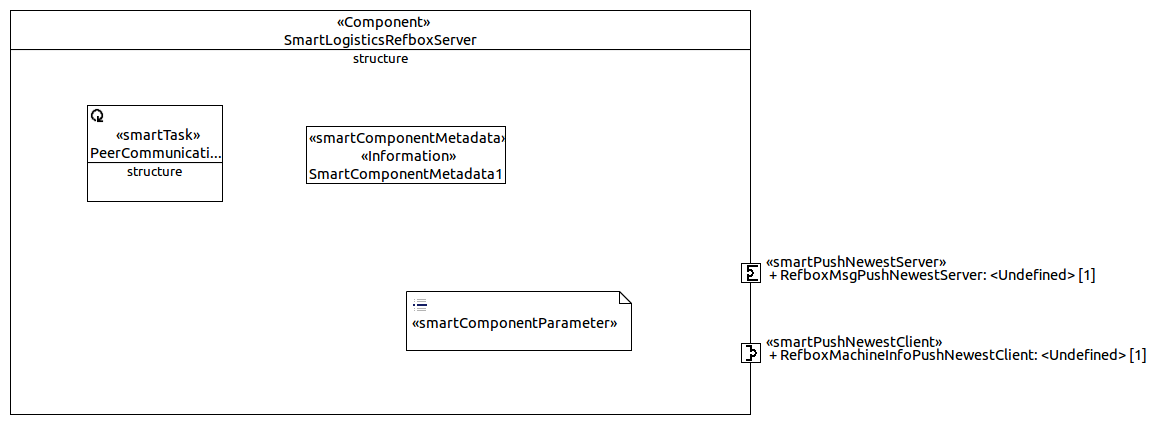
\includegraphics[width=\linewidth]{pic/component_refbox_server.png}
\caption{Model of Refbox server}
\label{fig:modelRefboxServer}
\end{figure}


\subsubsection{Configuration}

The component can be modified by the following parameters:
\begin{itemize}
\item \textbf{HostIP}, the IP address of the Referee Box
\item \textbf{Name}, the name of the robot, which is displayed on the Referee Box GUI
\item \textbf{Number}, the number of the robot, which is displayed on the Referee Box GUI
\item \textbf{Cryptokey} the key, which is used for the encrypted team channel
\end{itemize}

At the Robocup competition 2017 the hosts used AES with Electronic Codebook Encryption (ECB), while the Refbox in the laboratory used Cipher Block Chaining (CBC) for encryption. Therefor the team has to change the cipher method to the correct version at the competition.

	


\section{SmartRobotinoDetection}
	The detection of the MPS stations is an important part at the competition. This chapter gives detailed insights of the new implemented SmartRobotinoDetection component. 


\subsubsection{Overview}

The SmartRobotinoDetection component has only one task: it should detect the MPS stations near by the robot on the field. Therefor, if the component gets triggered, it commands the robot to perform a 360 degree turn and detect all the machines around.

\subsubsection{Old Version 2017}
The former team has implemented the SmartMPSDockingRoboCup component. 

\begin{figure}[h]
\centering
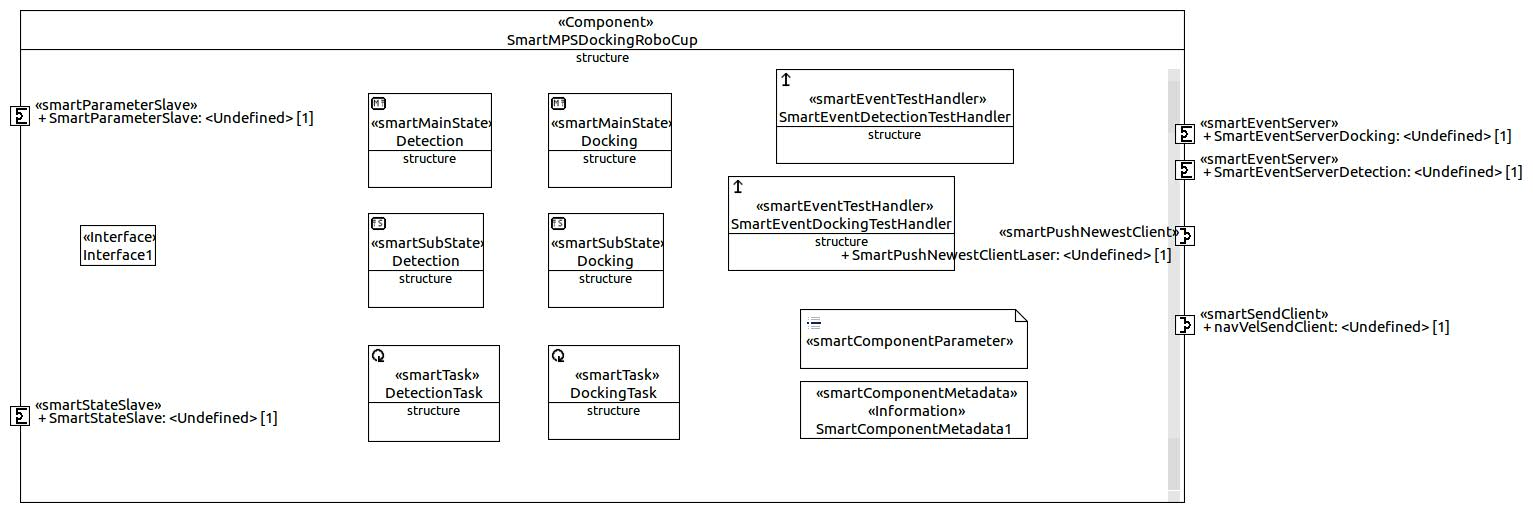
\includegraphics[scale=0.4]{pic/SmartMPSDockingRoboCup.jpg}
\caption{Model of MPS Detection/Docking Component}
\label{fig:dockingold_overview}
\end{figure}

Their idea was to combine the detection of the MPS stations and docking to the stations in one component. The detection worked most of the time, but the docking was completely random. This chapter just describes the detection part, and the docking is described in the next chapter. 
The combination of different tasks (detection and docking) contradict the idea of Smartsoft where concrete software components recommended. By splitting the detection from the docking, it would also be possible to replace on the fly the detection via the laser scanner by the detection via the camera, mounted on the robot.
Further the old SmartMPSDockingRoboCup component is implemented in a very confusing way and is hard to understand, so the team of 2018 decided to rewrite the component completely and discard the old one.


\subsubsection{ New Version 2018}

Each Skill component should satisfy one specific task. Therefor the new SmartRobotinoDetection component just detects MPS machines around the robot and the model is accordingly simple.

\begin{figure}[h]
\centering
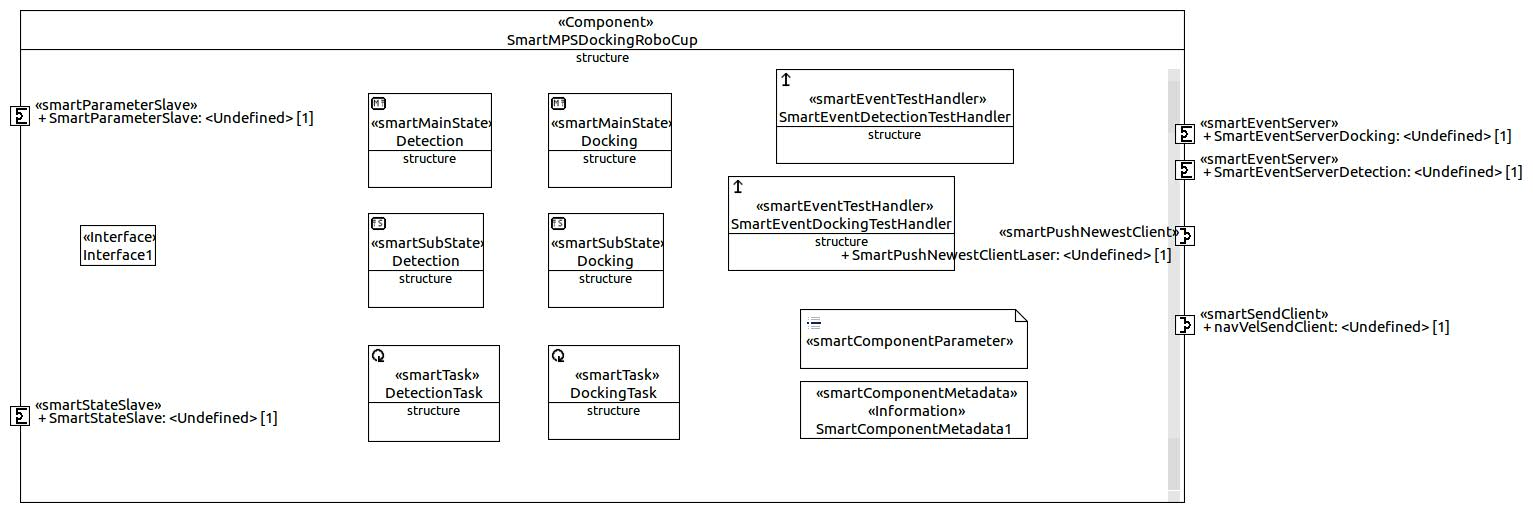
\includegraphics[scale=0.4]{pic/SmartMPSDockingRoboCup.jpg}
\caption{Model of MPS Detection/Docking Component}
\label{fig:dockingold_overview}
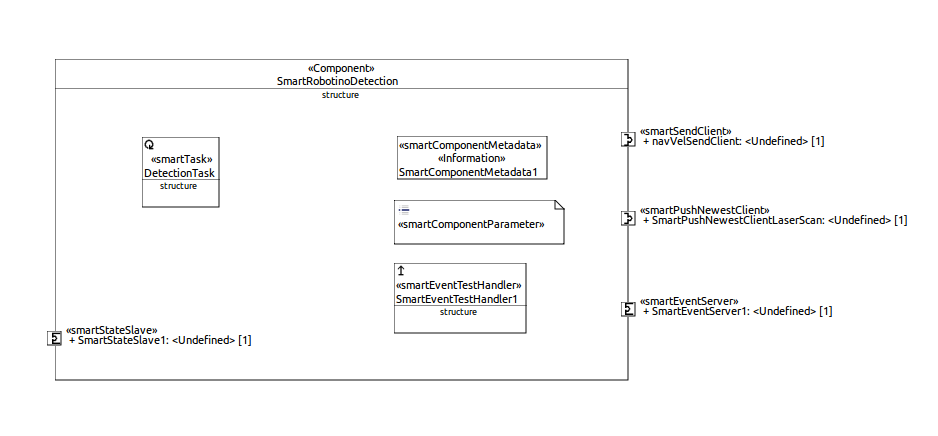
\includegraphics[scale=0.4]{pic/detectionComponent.png}
\caption{Model of MPS Detection Component}
\label{fig:dockingNew_overview}
>>>>>>> 015ec9cdd353798adb529438a628090223edc998
\end{figure}

The new detection component consists of one task (e.g. DetectionTask). If this task is triggered, the component commands the robot to perform a 360 degree turn at the current position. Every detected MPS station is sent back to the Sequencer, for further processing. 
The algorithm for the detection of the MPS station is more or less the same like the years before. But the verification of the detected MPS station has changed. The complete border of the field is excluded in the new version. Therefor it is not possible for the robot, to confuse the border of the field at the Robocup with a MPS machine. This simple approach lead into very good testing results. 

\paragraph{Detection Results}
The results are still sent via the old CommStationDetectionEventResult object, which contains 

\begin{enumerate}
\item MPSStationDetectionResult
\item CommMPSStationData (as a vector)
\end{enumerate}

The MPSStationDetectionResult is an enum which provides general information whether a MPS was found (MPS\_FOUND) or not (NO\_MPS\_FOUND).
The CommMPSStationData vector is empty if the component did not find any MPS stations. Because the docking algorithm of 2017 was very complicated, lots of information of the MPS station where needed. Thats why the CommMPSStationData contains lots of fields and seems bloated. It contains:

\begin{itemize}
\item orientation1 -> radial orientation corresponding to first docking point
\item orientation2 -> radial orientation corresponding to second docking point
\item centerX -> X coordinate of the MPS center point
\item centerY -> Y coordinate of the MPS center point
\item dockingPosX1 -> X coordinate of the first docking point
\item dockingPosX2 -> X coordinate of the second docking point
\item dockingPosY1 -> Y coordinate of the first docking point
\item dockingPosY2 -> Y coordinate of the second docking point
\item zone -> Zone of the Robocup map where the MPS resides
\end{itemize}

The new detection component uses the CommMPSStationData structure though, but just sets some of the parameters. For the new docking algorithm, just the corners of the appropriate stations are relevant, so the detection just writes the first corner in the dockingPosX1 and dockingPosY1. The second corner is written in the dockingPosX2 and dockingPosY2 fields. The rest of the parameters are ignored.

\paragraph{Configuration of the excluded Border}
The component can exclude the border of the field. Therefor some smartComponentParameters can be set in the component.
 
\begin{itemize}
\item xMin
\item yMin
\item xMax
\item yMax
\end{itemize}

Just define points in world coordinates, from where potential machines should be excluded.
It is necessary to adjust those parameters at the Robocup, because the Robocup field is much bigger than the testing field in the laboratory.
To switch the feature off, just set huge numbers for xMax and yMax, and very small numbers for yMin and yMin.








	
\section{SmartRobotinoMPSDocking}
	This section deals with the new SmartRobotinoMPSDocking component. The new docking algorithm is discussed in this chapter, including the advantages and disadvantages of the new approach.

\subsubsection{Overview}

The new docking approach is much more lightweight than the old one from 2017.

\begin{figure}[h]
\centering
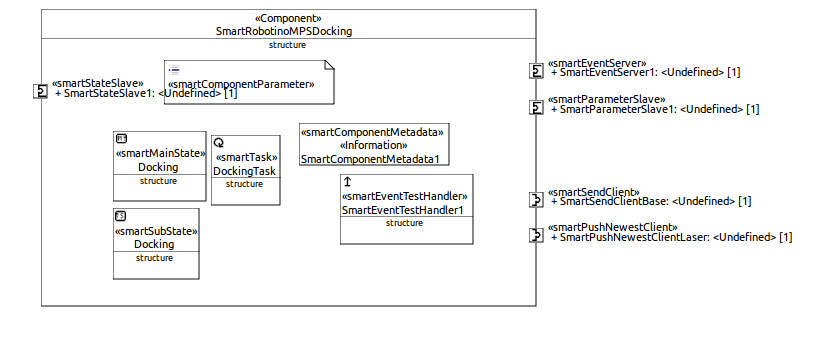
\includegraphics[scale=0.4]{pic/dockingComponent.png}
\caption{Model of the new Docking Component }
\label{fig:i_overview}
\end{figure}

The component consists mainly of one task (e.g. DockingTask), which just performs the docking to the corners of a MPS station, provided by the detection component.

\subsubsection{Old Version 2017}

The docking procedure of the former team was part of the SmartMPSDockingRoboCup component, which combined the detection task with the docking task.
The docking algorithm is implemented in a very incomprehensible way and also provides random docking results. Therefore the team of 2018 implemented a complete new docking component, which is lightweight, easy to understand and simple to optimize.

\subsubsection{New Version 2018}

For the new docking approach the two corners of the target MPS station is enough information. The docking task performs the following procedure:

\begin{enumerate}
\item Turn towards the target MPS station
\item Calculate the angle between robot and MPS station
\item Turn left or right until angle of robot to station is around 90 degree
\item Drive towards the middle of the MPS station, while angle to station is around 90 degree
\end{enumerate}

The calculation of the angle between robot and the target MPS station is described in the next paragraph. The other points of the procedure are descriptive to the enumeration above implemented.

\paragraph{Calculation of the angle between robot and MPS}

The corners of the target MPS station assemble a vector (e.g. stationVector). The robot has also a direction vector assigned, which is always pointing in the facing direction of the robot (e.g. roboDirectionVector). For the calculation of the angle between those two vectors, the well-known formula of the dot product of the two vectors divided with the length of the both vectors is used. To get always the acute angle of the vectors, the absolute value of the dot product is used. 

\begin{equation}
\cos(\phi) = \frac{ \vert \overrightarrow{roboDirectionVector} \circ \overrightarrow{stationVector} \vert} { \vert \overrightarrow{roboDirectionVector}  \vert  \cdot \vert \overrightarrow{stationVector}  \vert}
\end{equation}

\begin{equation}
\phi = \cos ^{ - 1} \left( \frac{ \vert \overrightarrow{roboDirectionVector} \circ \overrightarrow{stationVector} \vert} { \vert \overrightarrow{roboDirectionVector}  \vert  \cdot \vert \overrightarrow{stationVector}  \vert} \right)
\end{equation}


This approach only works, if the robot somehow faces the target MPS machine. Thats why the robot turns towards the target MPS station, before calculating the angle (robot - station). 

/// COMMUNICATION OBJECT /////

\paragraph{Optimizations}
Several optimizations can be done at the Robocup. 

\begin{enumerate}
\item Increase the speed of turning
\item Increase the speed of driving towards the center of the MPS station
\item Introduce a minimal and maximal distance to the MPS station (e.g. 1 meter), to stay in range for the ALVAR Tag detection
\end{enumerate}


\subsubsection{Summary}
The new docking component works very well. The approach is easy to extend and to optimize. It was not possible to reuse the old component smartMPSDockingRobocup, which combined detection with docking. It would have been to time consuming, finding all the bugs in the overcomplicated component. 


\chapter{Lessons learned}
    This section describes the facts which all the team members learned through development of the Robocup software. It describes the organization of the 
project team, what was wrong and what should be done better.

\subsection{Organization during the semester}
 
\subsubsection{Project Handover from the previous Team}

When the 2017 team took over the project from the 2016 seniors in autumn 2016, only a single remaining member of the 2016 team was available. This led to the fact that team members who took over a certain component didn't have a point to start. Although there were documentation like the book of knowledge \cite{BOK} and the 2016 tech report available, it was often not trivial to understand the intention of certain implementation details within the components. Therefore, it would be suggested to carry out a smooth project handover. This means that a senior member and a junior member work together for a certain amount of time. After this time, the junior member should understand the code and can implement some simple components by himself. \\

This was not the case in the 2016 to 2017 handover, so a lot of time was wasted due to reverse engineering and understanding certain components by the team members. 
 
\subsubsection{Meetings and assignments}
 
A software project should have regular meetings to make sure each member has the correct overview what he has to do within the project. At the beginning of the project, the junior team met with the last remaining senior member of the 2016 team to assign components to each new junior member. After this each member worked mostly by himself. This led to the fact that sometimes interfaces where not really clear between components which were developed by two independent members. After the arrival of new junior members in march 2017, a new meeting strategy was followed. On each Wednesday which was the working day for the Robocup team, a small meeting was scheduled in the morning before the team started to work on the project. This resulted in the situation that every team member had an overview of what all other team members were doing. Following this strategy faster progress could be made than within the first semester. Also tasks and deadlines (i.e. scrum sprints) were assigned to the team members. Although sometimes those tasks were not reached within a certain sprint, the overall performance improved.


\subsubsection{Testing}

Testing is an important thing which should not be neglected. The team tested the scenario in the lab but not with really great success. This was due to the fact that there were certain bugs within the components which often led to a stop of the integration testing until those bugs were fixed. Because of these issues, the team did not manage to have a complete running exploration phase before the Robocup. Also small remaining time prevented detailed testing before the Robocup. To avoid this in the future, teams should assign testing at least the same priority as development. Also if the whole exploration phase (or production phase in the future) can not be tested from the beginning, small tests between components should be made. This should lead to a more robust software and less time rush before the Robocup. \\

So the testing and bug-fixing was done mostly at the Robocup competition. It is the norm and very bad practice that the teams test and improve their software at the Robocup competition but the major testing and development should be done beforehand. 

 
\subsection{Organization for the competition}
 
As said before the team should have a running scenario when it arrives at the Robocup. This leads to a more relaxed competition and the team can concentrate on making small improvements to the software to perform well on the competition. It should be obvious that the rules of the annual Robocup change each year. Unfortunately, this was not really taken into account by the 2017 team. So the team was unprepared to new changes in the 2017 Magdeburg competition. To battle this issue certain changes were made to the Instruction Planner at the Robocup.  \\

To get around this issue the future team should study the Robocup Logistics League announcement so that adaptions to the new rules in the scenario can be made beforehand. A flexible software architecture may be a good idea so that new changes can be adapted quickly. There exists a mailing list of the Referee Box software which should be followed by the team so that always the newest version is used for development. \\

Also the team should fully understand the software it operates on the Robotino. There should be a team member who at least is an expert in one component. This means that the team can fix issues with their components independently from the lab team in the university. \\
 
At least one person of the team should act as a bridge between the Robocup staff and the team. This person should also be responsible for hotel booking and renting cars within a certain time range before the Robocup. By following these rules, the team should not have any issues with arriving and staying in Magdeburg. This team manager role relieves other team members from organizational stuff and they can focus on development and testing of the software.     
 


\chapter{Outcome}
    \section{Ideas for 2018}

The Robocup team 2017 has many ideas to improve the Robocup project for the next team.\\

The first idea is that the exploration of the field should be more efficient. In 2017, some fixed zones were explored. A first improvement can be to choose the nearest MPS station to approach. To realize this solution, all MPS stations already explored should be stored. A distributed database of detected stations can be a good solution even with multiple Robotinos. To recognize the tag, a perfect docking should be working. In the last version, some imperfections were problematic. Another solution can be to use a smart agent which explores the field. The solution should be able to find each MPS of the team in the limited time.\\

The second point is to use the three Robotinos in the field. Indeed, in 2017 only one robot was used. A multi-deployment is needed for this. A logic should be designed to interact with all these robots. The latest idea was to use one robot as a master and two robots as slaves. A better solution can be to have a peer to peer implementation. Each robot can be a smart agent and communicates with the others.\\

Another idea was to test more the deployment before the contest. It is necessary to drive around with robots and operate in the laboratory before the competition. The problem is that the field in the laboratory is smaller than the real field in the competition. To face this, the Gazebo simulator should be used. With the simulator, a real situation can be tested. A previous implementation was done by the 2016 team. This approach is available in the git repository.\\

An idea to have a better code can be to implement more using SmartTCL. To do this, a lot of effort should be put in the lisp language. One or two persons in the team need to know very well this language. \\

An important missing part during the contest was the production phase. Only the exploration phase was implemented in 2017. That's why the next task is to improve the exploration phase and to begin the production phase. It is important to be prepared for the future changes. Indeed, the contest becomes harder every year, so a good idea can be to imagine the next modification in the rules.\\

\printbibliography

\end{document}